\documentclass{article}

\usepackage{course_report}
\usepackage[utf8]{inputenc}
\usepackage[T1]{fontenc}
\usepackage{microtype}
\usepackage{graphicx}
\usepackage{booktabs}
\usepackage{array}
\usepackage{tabularx}
\usepackage{hyperref}
\usepackage{url}
\usepackage{amsmath}
\usepackage{amssymb}
\usepackage{mathtools}
\usepackage[capitalize,noabbrev]{cleveref}
\usepackage[round,authoryear]{natbib}

\hypersetup{colorlinks=true,linkcolor=black,citecolor=black,urlcolor=blue,pdftitle={Causal Disentanglement Across Data Regimes},pdfauthor={Kyung Wook Back}}
\graphicspath{{../figures/}}

\newcommand{\pa}{\operatorname{pa}}
\newcommand{\an}{\operatorname{an}}
\newcommand{\MMD}{\operatorname{MMD}}
\newcommand{\Cov}{\operatorname{Cov}}
\newcommand{\rank}{\operatorname{rank}}

\title{Causal Disentanglement Across Data Regimes}

\author{%
  Kyung Wook Back\\
  Department of Statistics, Korea University\\[0.5em]
  \normalfont Advanced Machine Learning course project, Spring 2026
}

\begin{document}
\maketitle

\begin{abstract}
This course project compares three identifiability results for causal disentanglement: from purely observational data \citep{welch2024observational}, from unpaired soft interventions \citep{zhang2023soft}, and from one perfect intervention per latent node in a linear model \citep{squires2023linear}. It compares their assumptions, the objects they identify, and the observable signal each proof relies on. Three small synthetic experiments examine these signals at finite sample size: leaf selection from a noisy score Hessian, ancestor ranking from one-dimensional distribution shifts, and the rank-two structure of precision-matrix differences. The first two use known latent coordinates; the third estimates precisions after linear mixing. On the public scPerturb distribution of the Norman Perturb-seq data, additive composition of single-perturbation effects improves over the control predictor for 121 of 131 double perturbations. All ten negative-$R^2$ cases have predicted-to-observed norm ratios above $1.7$, including five with squared direction cosine above $0.7$. Raw expression correlations are uniformly high ($0.939$--$0.998$) and have only a modest association with prediction accuracy (Spearman correlation $0.362$ with $R^2$).
\end{abstract}

\section{Introduction}

Causal representation learning starts from high-dimensional measurements $X$, such as gene-expression vectors, and posits a low-dimensional latent system $Z$ whose coordinates are related by an unknown DAG $\mathcal G$:
\begin{equation}
    X=f(Z),
    \qquad
    P(Z)=\prod_{i=1}^{d} P\!\left(Z_i\mid Z_{\pa_{\mathcal G}(i)}\right).
    \label{eq:common-setup}
\end{equation}
Both the coordinates and the graph must be inferred. Because $f$ is unknown, a reparameterized latent vector can often be absorbed into a different mixing map without changing the distribution of $X$, so the question is which causal object is identifiable, and up to which equivalence, from the data at hand. At minimum latent labels can be permuted, and most models also allow componentwise affine maps $\widehat Z_i=a_iZ_{\pi(i)}+b_i$ with $a_i\neq0$.

Interventional data reduce this ambiguity because one mixing map must explain several related distributions. A soft intervention on node $i$ replaces $P(Z_i\mid Z_{\pa(i)})$ by another conditional $P^{I_i}(Z_i\mid Z_{\pa(i)})$ that may still depend on the parents. A perfect intervention removes the parent dependence and leaves $Z_i$ stochastic, $P^{I_i}(Z_i)$. The three papers studied here sit at increasing levels of intervention: \citet{welch2024observational} use $P_X$ alone and recover causal layers; \citet{zhang2023soft} use unpaired soft-interventional contexts and recover ancestral relations; \citet{squires2023linear} use one perfect intervention per node in a linear model and recover the full latent DAG. Each result combines its data regime with a different set of assumptions on the latent mechanisms, mixing map, and faithfulness.

The report follows the theoretical comparison with two empirical analyses. \Cref{sec:results} summarizes the three results and tabulates their assumptions, identifiable objects, and identifying signals. \Cref{sec:synthetic} runs one small simulation per regime that isolates that signal under oracle information. \Cref{sec:norman} evaluates additive prediction of double perturbations on the Norman Perturb-seq data and decomposes the error into direction and magnitude. 

\section{Three Identifiability Results}
\label{sec:results}

\subsection{Observational data: causal layers}

\citet{welch2024observational} consider injective linear mixing of a nonlinear additive Gaussian latent model,
\begin{equation}
    X=HZ,
    \qquad
    Z_i=f_i(Z_{\pa(i)})+E_i,
    \qquad E_i\sim\mathcal N(0,\sigma_i^2).
    \label{eq:obs-model}
\end{equation}
The result also assumes that the nonconstant mechanisms are nonlinear in every parent-space direction. Nodes are grouped into causal layers: layer $0$ holds the leaves, and layer $k$ holds nodes whose longest directed path to a leaf has length $k$. From $P_X$ alone, each latent coordinate is identified only up to a linear combination of variables in its own and upstream layers, and the paper shows that no finer recovery is possible in general.

The identifying signal is the Hessian of the log density, $J_X(x)=\nabla_x^2\log p_X(x)$, which transforms as $J_Z(z)=H^\top J_X(x)H$ under linear mixing. In the additive Gaussian model the diagonal Hessian entry of a leaf is constant, $-1/\sigma_i^2$, whereas the entry of a non-leaf node varies with $z$ through its children's mechanisms. The algorithm estimates $J_X$, finds directions with near-zero variance of the diagonal entry by solving quadratically constrained quadratic programs, removes that layer, and repeats. Second-order score estimation and the nonconvex optimization are the practical bottlenecks.

\subsection{Soft interventions: ancestral relations}

\citet{zhang2023soft} observe unpaired samples from an observational distribution and from atomic soft interventions, with at least one intervention per latent node. Under a polynomial mixing class that reduces to an unknown linear map, and a generalized interventional faithfulness condition, the marginal changes identify ancestral relations among the intervention targets, that is, the transitive closure of the latent graph. A further conditional-faithfulness assumption identifies the DAG and intervention targets up to a common permutation. The constructive proof selects a sparsest compatible representation. General soft interventions still leave ambiguity in the latent coordinates. The signal is that an intervention on $Z_i$ changes the marginal of every descendant,
\begin{equation}
    i\in\an(j)
    \quad\Longrightarrow\quad
    P(Z_j)\neq P^{I_i}(Z_j),
    \label{eq:desc-shift}
\end{equation}
and leaves other non-descendants unchanged; faithfulness rules out cancellations. The synthetic probe below assumes these coordinates are known; the theorem must also resolve their unknown mixing. The estimator is a variational autoencoder whose decoder generates interventional samples from a learned latent SCM and matches them to the real interventional samples by maximum mean discrepancy (MMD), with a sparsity penalty on the latent adjacency. Its output depends on optimization, latent dimension, and intervention strength.

\subsection{Perfect interventions: the full latent DAG}

\citet{squires2023linear} study a linear Gaussian latent SCM with linear injective mixing,
\begin{equation}
    Z=A_kZ+\Omega_k^{1/2}\epsilon,
    \qquad X=GZ,
    \qquad \epsilon\sim\mathcal N(0,I),
    \label{eq:perfect-model}
\end{equation}
over an observational context and single-node interventional contexts. A perfect intervention on node $i$ zeroes row $i$ of $A_k$ and assigns a parent-independent noise distribution. With one informative intervention per latent node, the graph, targets, and parameters are identified up to a graph-compatible permutation after fixing the latent scale and sign conventions; if some node is never intervened on, distinct models can be indistinguishable. Since $p>d$ makes $\Cov(X)$ singular, the paper works with pseudoinverse precisions $\Theta_k=\Cov(X_k)^\dagger$. A single-node intervention changes one latent mechanism, so
\begin{equation}
    D_k=\Theta_k-\Theta_0,
    \qquad \rank(D_k)\leq 2,
    \label{eq:rank-two}
\end{equation}
with rank one for a source node under genericity. The row spaces of the $D_k$ give the partial order and the mixing matrix through RQ and Cholesky decompositions. This result requires linear mechanisms and mixing, together with one selective perfect intervention per latent node. The rank bound itself also holds for single-node soft interventions in the linear model; rank alone does not distinguish the two.

\subsection{Comparison}

\Cref{tab:comparison} places the three results side by side. They take different inputs and identify different objects (a layer partition, a set of ancestral relations, a DAG), so there is no single score on which to compare them; projecting a DAG estimate to layers discards identified edges, and scoring a layer estimate by structural Hamming distance penalizes edges that $P_X$ cannot identify. The experiments below therefore score each signal against its own target. Estimation cost also does not follow the ordering: the observational method needs second-order score estimates and repeated nonconvex solves, the soft method needs neural optimization and quadratic-cost kernel sums, and the perfect-intervention method is algebraic once covariances are estimated.

\begin{table}[t]
\centering
\caption{The three identifiability results.}
\label{tab:comparison}
\begingroup
\footnotesize
\setlength{\tabcolsep}{3pt}
\renewcommand{\arraystretch}{1.18}
\begin{tabularx}{\textwidth}{@{}l >{\raggedright\arraybackslash}p{0.13\textwidth} >{\raggedright\arraybackslash}p{0.21\textwidth} >{\raggedright\arraybackslash}X >{\raggedright\arraybackslash}p{0.18\textwidth}@{}}
\toprule
\textbf{Regime} & \textbf{Data} & \textbf{Model and mixing} & \textbf{Observable signal $\boldsymbol{\rightarrow}$ identifiable object} & \textbf{Main bottleneck} \\
\midrule
Observational & $P_X$ only & directionally nonlinear additive Gaussian; injective linear mixing & score-Hessian variation $\rightarrow$ upstream-layer representations & second-order score estimation \\
\addlinespace[0.15em]
Soft & unpaired $P_X,P_X^{I_k}$; all targets covered & general SCM; full-rank polynomial mixing & marginal shifts $\rightarrow$ ancestry; DAG and targets under stronger faithfulness & faithfulness and VAE optimization \\
\addlinespace[0.15em]
Perfect & observational plus single-node contexts & linear Gaussian SCM; linear mixing & rank-$\leq2$ precision differences $\rightarrow$ full latent DAG & model mismatch and finite-sample rank testing \\
\bottomrule
\end{tabularx}
\endgroup
\end{table}

\section{Synthetic Experiments}
\label{sec:synthetic}

All three experiments use the five-node graph
\begin{equation}
    Z_1\to Z_2,\quad Z_1\to Z_3,\quad
    Z_2\to Z_4,\quad Z_3\to Z_4,\quad Z_4\to Z_5,
    \label{eq:shared-dag}
\end{equation}
with layers $L(Z_5)=0$, $L(Z_4)=1$, $L(Z_2)=L(Z_3)=2$, $L(Z_1)=3$, but each uses its own data-generating process matching its regime's assumptions. The observational and soft probes work in the true latent coordinates. The perfect-intervention probe computes precision differences in the mixed observations $X=GZ$. Seeds, grids, and per-repetition outputs are recorded with the results.

\begin{figure}[t]
    \centering
    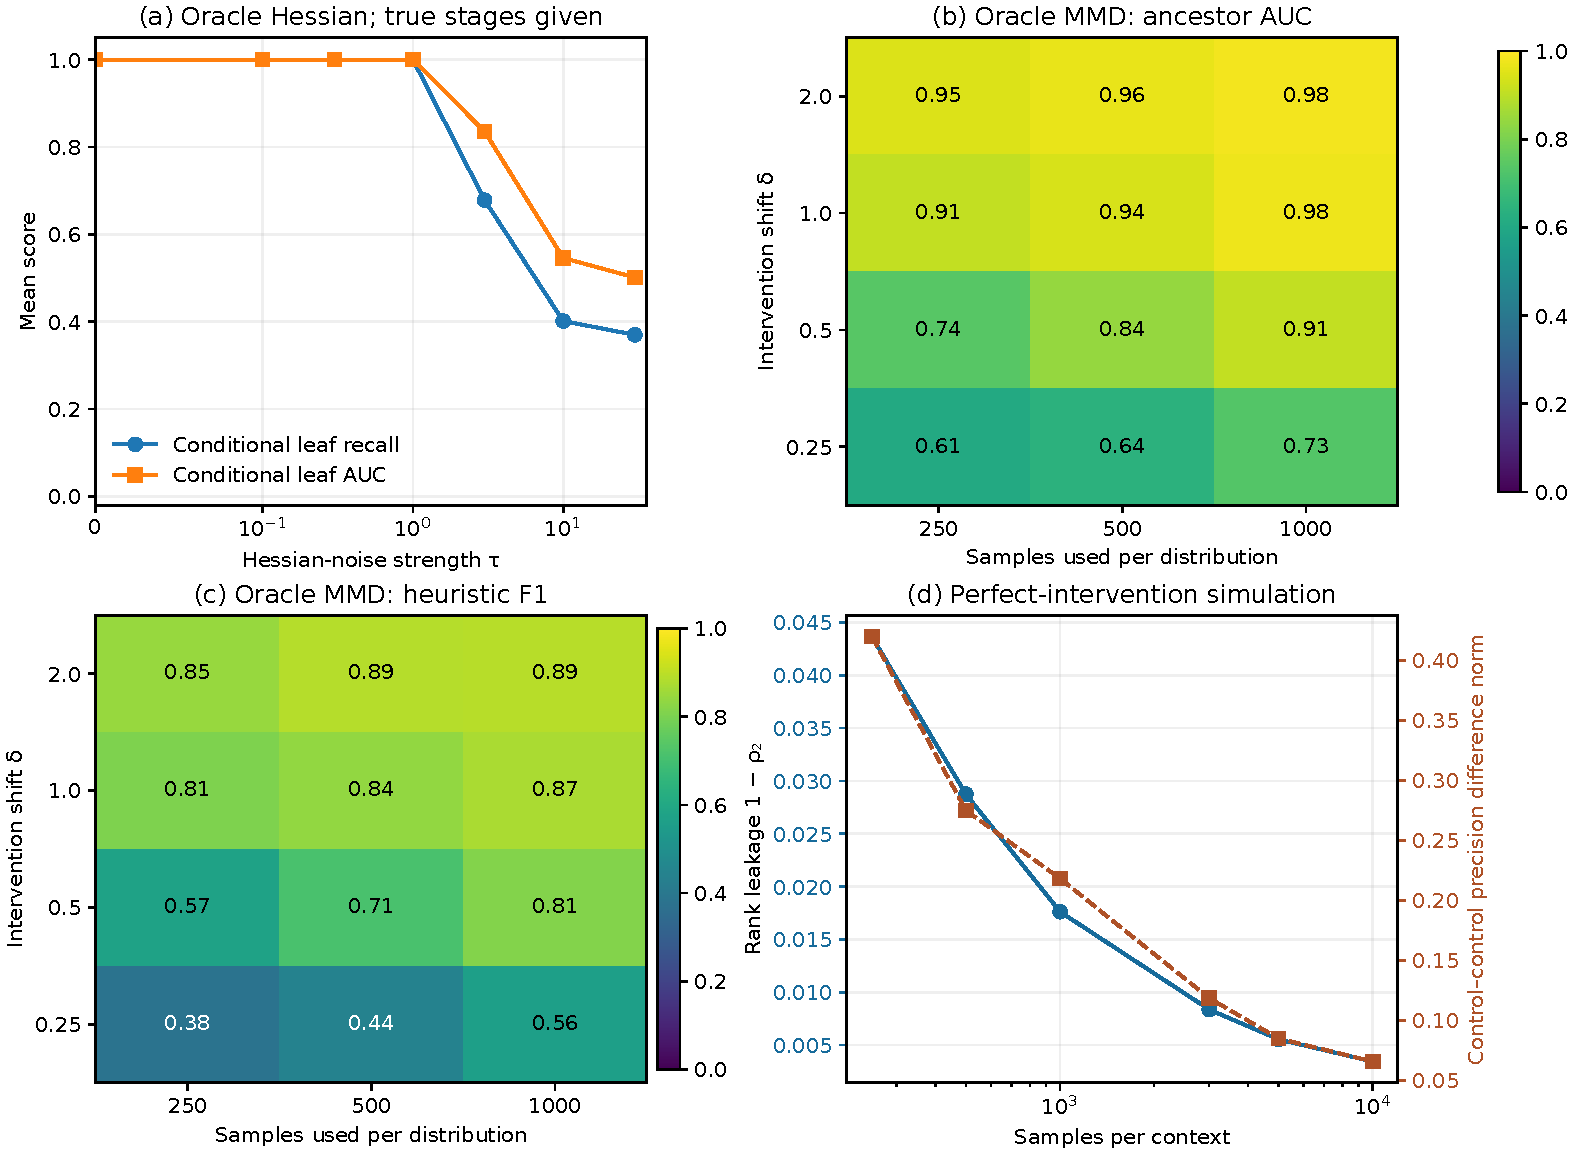
\includegraphics[width=\textwidth]{synthetic_probes.pdf}
    \caption{Synthetic experiments. (a) Leaf recall and leaf AUC at the true peeling stages as noise is added to the oracle score Hessian (200 repetitions, $n=300$). (b, c) Ancestor AUC and heuristic ancestral-pair $F_1$ from one-dimensional MMD shifts, by sample size and shift $\delta$ (30 repetitions). (d) Rank leakage $1-\rho_2$ of intervention precision differences and the Frobenius norm of a control-versus-control difference, by samples per context (50 repetitions).}
    \label{fig:synthetic}
\end{figure}

\subsection{Observational: leaf selection from a noisy score Hessian}

The mechanisms combine $\tanh$, $\sin$, and quadratic terms of the parents with Gaussian noise, so the model is of the form in \cref{eq:obs-model}. The diagonal entries of the latent score Hessian are computed analytically for each sample, and independent Gaussian noise is added to those diagonal entries, $\widehat J_{jj}(z)=J_{jj}(z)+\tau s W_j(z)$ with $W_j(z)\sim\mathcal N(0,1)$. Here $s$ is the median sample standard deviation of the true non-leaf entries at that stage. At each peeling stage the set of remaining nodes and the number of leaves to remove are taken from the true layers; the nodes with the smallest empirical variance of their diagonal entry are selected as leaves. The final stage, where only $Z_1$ remains, has nothing to compare and is skipped. Two scores are averaged over the three remaining stages: leaf recall of the selected set and the AUC of the variance ranking against the true leaf labels. Each of the 200 repetitions draws a new sample of $n=300$; the $\tau$ settings within a repetition share the data and the noise realization.

\Cref{fig:synthetic}a shows both scores at $1.0$ for $\tau\leq1$. At $\tau=3$ recall is $0.68$ and AUC $0.84$; at $\tau=10$ they are $0.40$ and $0.55$, and at $\tau=30$ the AUC is $0.50$, chance level.

\subsection{Soft interventions: ancestor ranking from marginal shifts}

An intervention on target $i$ adds $\delta$ to the exogenous noise of $Z_i$ and keeps the parent mechanism, a shift intervention. For an ordered pair $(i,j)$ with $i\neq j$ the score is the squared RBF MMD between the observational and interventional samples of the single coordinate $Z_j$,
\begin{equation}
    S_{ij}=\MMD^2\!\left(P(Z_j),P^{I_i}(Z_j)\right),
\end{equation}
computed as the biased V-statistic over all $n$ samples of each distribution. The RBF bandwidth is set from the median pairwise squared distance among at most 400 pooled samples. The label is whether $i$ is an ancestor of $j$ in \cref{eq:shared-dag}, giving 9 positives among 20 pairs. Two scores are reported: the threshold-free ancestor AUC, and the $F_1$ of pairwise ancestry predictions obtained by declaring $i\in\an(j)$ when $S_{ij}$ exceeds the 95\% quantile of five control-versus-control scores (one per coordinate) computed from two independent observational samples. The cutoff uses NumPy's linearly interpolated quantile. Predicted pairs are scored directly without enforcing transitivity. The grid is $n\in\{250,500,1000\}$, $\delta\in\{0.25,0.5,1,2\}$, 30 repetitions.

The AUC in \cref{fig:synthetic}b rises with both $n$ and $\delta$: at $\delta=0.25$ it goes from $0.61$ to $0.73$ as $n$ grows from 250 to 1000, at $\delta=1$ from $0.91$ to $0.98$, and at $\delta=2$ it is $0.95$ already at $n=250$. The heuristic $F_1$ in \cref{fig:synthetic}c follows the same ordering but stays lower, from $0.38$ at the weakest setting to $0.89$ at $\delta=2$, $n=1000$. In this SCM, stronger shifts and more samples improve marginal-shift ranking in the supplied coordinates.

\subsection{Perfect interventions: rank of precision differences}

A linear Gaussian SCM with $d=5$ latent and $p=10$ observed variables follows \cref{eq:perfect-model}, with edge weights drawn uniformly in magnitude from $[0.35,0.9]$ with random sign, noise variances in $[1,2]$, and a mixing matrix with orthogonal columns scaled in $[0.8,1.5]$. A perfect intervention on target $i$ zeroes row $i$ of $A$ and multiplies the noise variance of $Z_i$ by $4$. Each context's precision is the pseudoinverse of its sample covariance, truncated at relative eigenvalue $10^{-10}$; no ridge is added, because inverting a ridge in the five-dimensional null space produces large eigenvalues whose cancellation would dominate the differences. For $D_k=\widehat\Theta_k-\widehat\Theta_0$ the statistic is the share of squared singular-value energy in the top two directions,
\begin{equation}
    \rho_2(D_k)=
    \frac{\sigma_1^2(D_k)+\sigma_2^2(D_k)}
         {\sum_r\sigma_r^2(D_k)},
    \qquad
    \text{leakage}=1-\rho_2(D_k),
    \label{eq:rho2}
\end{equation}
$\rho_2$ equals one in population by \cref{eq:rank-two}. Leakage is averaged over the five targets within each of 50 repetitions, each with freshly drawn parameters, for $n\in\{250,500,1000,3000,5000,10000\}$ samples per context. As a null, the Frobenius norm of the difference between two independent control precision estimates is also recorded.

Mean leakage falls from $0.044$ at $n=250$ to $0.0035$ at $n=10{,}000$ (\cref{fig:synthetic}d), while the control-control norm falls from $0.42$ to $0.066$ and the intervention-difference norm stays near $0.7$--$0.8$. The rank-two structure is thus already dominant at $n=250$ in this model and sharpens with $n$.

\section{Norman Perturb-seq: Additive Prediction of Double Perturbations}
\label{sec:norman}

\subsection{Data}

The Norman et al.\ experiment \citep{norman2019exploring} measures single-cell transcriptomes under CRISPR activation of one or two genes (GEO GSE133344). This analysis uses the scPerturb distribution \citep{scperturb2022data}, with 111,445 cells and 33,694 genes: 11,855 control cells, 57,831 single-perturbation cells, and 41,759 double-perturbation cells. All cells in the supplied filtered file are retained. Counts are normalized to 10,000 per cell and log-transformed with $\log(1+x)$. The 2,000 genes with greatest variance are selected from a random sample of 50,000 control and single-perturbation cells, with seed 0. Double-perturbation cells are reserved for evaluation. Requiring at least 200 control cells, 50 cells per single perturbation, and 30 cells per double perturbation leaves 105 singles and 131 doubles, each with both constituent singles available. All prediction metrics use the same selected genes.

\subsection{Additive prediction and its decomposition}

Let $\mu^0$ be the control mean-expression vector, $\mu^i$ and $\mu^j$ the means under two single perturbations, and $\mu^{ij}$ the mean under their double. The two predictors compared are
\begin{equation}
    \widehat\mu^{ij}_{\mathrm{ctrl}}=\mu^0,
    \qquad
    \widehat\mu^{ij}_{\mathrm{add}}=\mu^i+\mu^j-\mu^0,
    \label{eq:norman-additive}
\end{equation}
scored by squared error relative to the double's deviation from control,
\begin{equation}
    R^2_{\mathrm{mean}}
    =1-\frac{\lVert \mu^{ij}-\widehat\mu^{ij}\rVert_2^2}
             {\lVert \mu^{ij}-\mu^0\rVert_2^2},
    \label{eq:norman-r2}
\end{equation}
so that the control predictor scores $0$ and negative values mean the additive estimate is worse than ignoring the perturbation. RMSE, the raw Pearson correlation between predicted and observed mean vectors, and $R^2$ on the 100 genes with the largest double-versus-control change were also computed; the last uses the observed double to pick the gene subset.

To separate direction from scale, write the observed and predicted effects $\delta^{ij}=\mu^{ij}-\mu^0$ and $\widehat\delta^{ij}=\widehat\mu^{ij}_{\mathrm{add}}-\mu^0$, their norm ratio $a=\lVert\widehat\delta^{ij}\rVert/\lVert\delta^{ij}\rVert$, and their cosine $c$. Expanding \cref{eq:norman-r2} gives
\begin{equation}
    R^2_{\mathrm{mean}}=2ac-a^2,
    \label{eq:direction-magnitude}
\end{equation}
For $c\geq0$, the best norm ratio at that direction is $a=c$. More generally, optimizing an unrestricted signed scalar multiplying the predicted effect gives $R^2_{\mathrm{scaled}}=c^2$. This scalar uses the observed double and serves only to separate direction error from scale error.

\subsection{Results}

The additive predictor beats the control predictor for 121 of the 131 pairs, with median $R^2_{\mathrm{mean}}=0.788$ and mean $0.592$. The median raw Pearson correlation is $0.991$, and the median top-100 $R^2$ is $0.908$. In effect space, the median cosine is $c=0.919$, with 18 pairs above $0.95$. Predicted norms exceed observed norms in 83 pairs; the median norm ratio is $a=1.097$. The median oracle-rescaled score $c^2$ is $0.845$. \Cref{fig:norman} shows how direction and magnitude jointly determine the prediction error.

All ten pairs with $R^2<0$ have $a>1.7$; five retain $c^2>0.7$. Five of the ten involve CEBPE. Across all 131 pairs, $a$ is positively associated with the sum of the two single-effect norms, $\lVert\mu^i-\mu^0\rVert+\lVert\mu^j-\mu^0\rVert$ (Spearman correlation $0.509$). Raw Pearson correlations range from $0.939$ to $0.998$, with Spearman correlation $0.362$ with $R^2$. Thus a high raw correlation provides limited discrimination among these predictions. CEBPE+KLF1 combines direction error ($c=0.596$) and magnitude error ($a=2.155$), giving $R^2=-2.072$.

\begin{figure}[t]
    \centering
    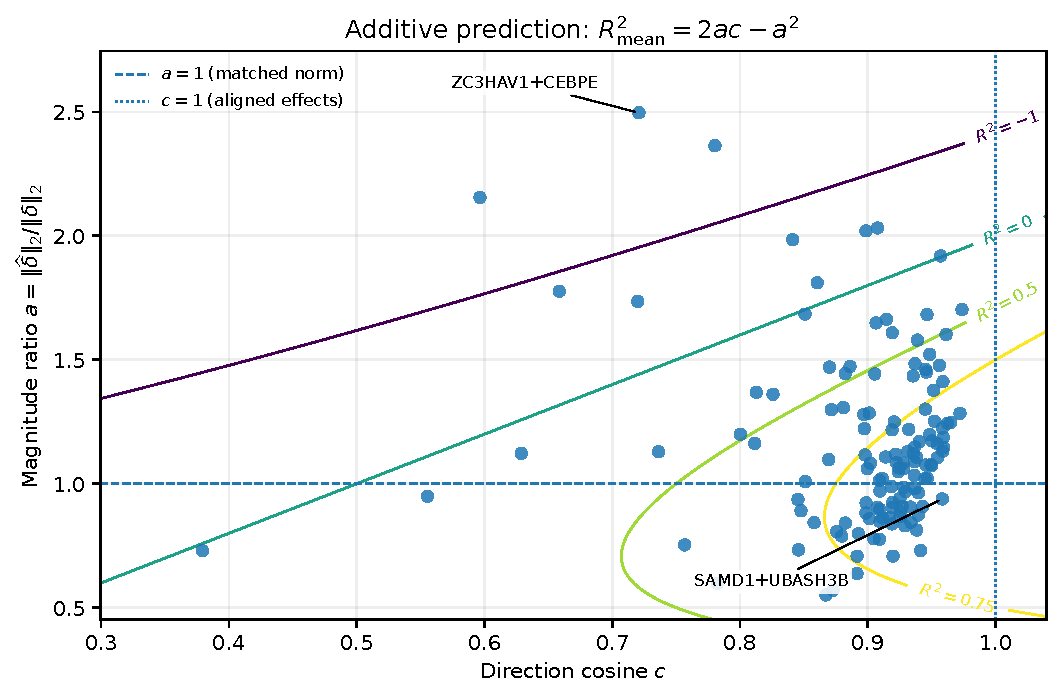
\includegraphics[width=0.82\textwidth]{norman_direction_magnitude.pdf}
    \caption{The 131 double perturbations by effect-direction cosine $c$ and norm ratio $a$. Contours are $R^2_{\mathrm{mean}}=2ac-a^2$; the dashed line is $a=1$ and the dotted line $c=1$. Predicted norms exceed observed norms for 83 pairs. The labeled pairs have the highest and lowest $R^2$.}
    \label{fig:norman}
\end{figure}

\section{Discussion}

The three synthetic experiments show how the identifying signals respond to noise, intervention strength, and sample size. Leaf ranking deteriorates under large Hessian perturbations, marginal shifts become easier to detect with stronger interventions, and precision differences concentrate near rank two as covariance estimates improve. The probes use oracle information to isolate these signals. Recovering latent coordinates, estimating a Hessian from observations, and propagating errors through successive layers remain tasks for the full estimators. The soft probe's $F_1$ uses only five null scores to set a cutoff; it is an exploratory summary without a calibrated false-positive rate.

Additive composition predicts most Norman double-perturbation responses well. Its failures cluster among large norm overestimates, and half of the negative-$R^2$ cases retain $c^2>0.7$. The association between larger single effects and norm overestimation motivates examining saturation of the combined response. Both quantities depend on the single-effect estimates, however, so their correlation alone cannot distinguish saturation from estimation effects. Reporting the direction cosine and norm ratio shows where each prediction goes wrong, while raw expression correlation remains high across the cohort. Appendix~\ref{app:rho2} examines the precision-difference signal on the same data.

The next step is to quantify uncertainty in these diagnostics by resampling cells within contexts and to assess sensitivity to the gene set. The current results describe one cell line under one preprocessing choice. In the synthetic experiments, varying the graph and its mechanisms would show how much of each trend extends beyond the five-node example.

\section*{LLM Use Disclosure}
Generative AI tools assisted with language editing, code review and corrections, test execution, and restructuring the report during revision. The author is responsible for the final content and interpretation.

{\small
\bibliographystyle{plainnat}
\bibliography{references}
}

\appendix

\section{Precision-Difference Concentration on the Norman Data}
\label{app:rho2}

For the 105 eligible single perturbations, expression profiles are projected to 20 centered principal components fitted to control and single-perturbation cells. Ledoit--Wolf shrinkage precisions $\widehat\Theta_i$ and $\widehat\Theta_0$ are estimated for each perturbation and for control, and $\rho_2(\widehat\Theta_i-\widehat\Theta_0)$ is computed as in \cref{eq:rho2}. The median is $0.570$, the mean $0.564$, and the range $0.367$--$0.850$. The linear single-target model gives a population precision-difference rank of at most two, including after a common fixed linear projection when precisions are defined on the shared covariance support. Hence $\rho_2=1$ whenever the difference is nonzero. A single control--control split into 5,928 and 5,927 cells (seed 0), using the same PCA coordinates and precision estimator, gives $\rho_2=0.501$. The single-perturbation contexts contain 113--1,960 cells. These unequal group sizes make the control split a descriptive reference. Per-perturbation values and the control split are included with the analysis results.

\section{Reproducibility}

The repository contains the three synthetic scripts, the Norman pipeline, the Norman context means and result tables, and the figure-generation code. Each synthetic run writes per-repetition results, a summary, and a settings file recording the grid, seed ($20260607$), and package versions. The figure command recomputes synthetic summaries from the per-repetition files and Norman pair metrics from the context means. The Norman pipeline accepts a processed AnnData file or the GEO filtered matrix, records the input checksum and all thresholds, and has a generated-data self-test. A downloader retrieves the scPerturb input from Zenodo and checks its checksum. The cell-level file itself is downloaded separately.

\end{document}
